\documentclass[11pt,a4paper]{article}
\usepackage[T1]{fontenc}
\usepackage{lmodern,microtype}
\usepackage[margin=25mm]{geometry}
\usepackage{amsmath,amssymb,amsthm,mathtools,bm}
\usepackage{graphicx,booktabs,tabularx,longtable,array}
\usepackage[dvipsnames]{xcolor}
\usepackage[round,authoryear]{natbib}
\usepackage{enumitem,caption,fancyhdr,xurl}
\definecolor{plum}{HTML}{754568}
\definecolor{jade}{HTML}{427F72}
\usepackage[colorlinks=true,linkcolor=plum,citecolor=jade,urlcolor=plum]{hyperref}
\hypersetup{pdftitle={An exact projected-angle likelihood and population inversion for wide-binary eccentricities},pdfauthor={Anonymous}}
\setlength{\parindent}{0pt}
\setlength{\parskip}{5pt}
\setlength{\headheight}{14pt}
\pagestyle{fancy}\fancyhf{}
\fancyhead[L]{\small Exact wide-binary angle laws}
\fancyhead[R]{\small Evidence Press candidate -- 31 October 2026}
\fancyfoot[C]{\thepage}
\captionsetup{font=small,labelfont=bf}
\setlist{itemsep=2pt,topsep=3pt}
\newtheorem{theorem}{Theorem}[section]
\newtheorem{proposition}[theorem]{Proposition}
\newtheorem{corollary}[theorem]{Corollary}
\newtheorem{lemma}[theorem]{Lemma}
\theoremstyle{remark}\newtheorem{remark}[theorem]{Remark}
\DeclareMathOperator{\acosh}{acosh}
\DeclareMathOperator{\atanh}{atanh}
\DeclareMathOperator{\TV}{TV}
\DeclareMathOperator{\Var}{Var}
\newcommand{\E}{\mathbb E}
\newcommand{\Prob}{\mathbb P}
\newcommand{\ind}{\mathbf 1}
\newcommand{\dd}{\,\mathrm d}
\title{\textbf{An exact projected-angle likelihood and population\\inversion for wide-binary eccentricities}}
\author{Anonymous}
\date{31 October 2026\\[2pt]\small Version 1.0.0-candidate. DOI: \href{https://doi.org/10.5281/zenodo.23838665}{10.5281/zenodo.23838665}}
\begin{document}
\maketitle
\vspace{-1em}
\begin{abstract}
A wide binary star takes thousands of years to complete one orbit, so its eccentricity usually cannot be found by following the orbit. Astronomers instead use the angle $\Gamma$ between the pair's projected separation and projected relative velocity, whose distribution over many binaries depends on the population's eccentricity law. In the ideal model, orbital phase is a random time in the orbit and orientation is uniformly random in three dimensions. For this model we derive the likelihood in closed form, $p(\gamma\mid e)=[\acosh(1/e)-\ind_{|\cos\gamma|>e}\acosh(|\cos\gamma|/e)]/(\pi\sin^2\gamma)$, and show that its mixtures are classical Abel transforms. This gives an explicit inverse for the population law, including atoms, and answers the uniqueness question raised in Appendix B of Hwang, Ting and Zakamska (2022): different eccentricity laws never give the same angle law. The inverse is continuous in the weak topology but discontinuous in total variation, so fine structure can be nearly invisible. Moments need no inversion: for example $\E\sqrt{1-e^2}=\tfrac\pi2\E\sin^3\Gamma$ and $\E e^2=\tfrac12+\E\cos2\Gamma-\tfrac12\E\cos4\Gamma$. These are the only symmetric unbiased single-angle observables for their targets, and they give near-efficient estimators of power-law indices. Two exact selection results bear on Gaia samples. Populations that are thermal at each semimajor axis and total mass keep a uniform angle law under selection on true lengths, line-of-sight angles, semimajor axis and total mass that ignores sky position angles. Binning by projected separation preserves the model when semimajor axes follow a scale-free log-uniform (\"Opik) law independent of orbital shape, phase and orientation. Simulations of Kepler orbits check representative formulas. No observational catalogue is analysed.
\end{abstract}

\smallskip
\textbf{Status and transparency.} This is an unrefereed Evidence Press candidate. It contains complete written proofs and reproducible synthetic checks. Development and checking were AI-assisted, including an internal multi-reviewer critique and an independent replay of all code. This is not external peer review, and no proof assistant was used. A documented literature search found no equivalent result; priority remains a bounded judgement.

\smallskip
\noindent\fbox{\parbox{0.97\linewidth}{\small\textbf{In plain terms.} Picture many binary stars, each caught at a random moment of its orbit and seen from a random direction. For each one we measure only the angle between the line joining the two stars and the direction in which they are moving relative to each other. This paper gives the exact probability of every such angle for an orbit of any shape (Section~\ref{sec:kernel}). It proves that the full distribution of angles pins down the population's eccentricities completely (Section~\ref{sec:inverse}), although fine detail is almost invisible (Section~\ref{sec:stability}). It also supplies simple averages of the angle that estimate useful summaries directly, such as the mean square eccentricity and the power-law index (Sections~\ref{sec:moments}--\ref{sec:ecc}). Finally, it says which common ways of selecting stars keep these results exact (Section~\ref{sec:selection}). Everything assumes ideal sampling, and no real catalogue is analysed here.}}

\section{The question and the contribution}

The eccentricities of wide binaries record how they formed and what has happened to them since. Pairs formed by the capture of unrelated stars or by dynamical relaxation tend towards the ``thermal'' law $f(e)=2e$ \citep{Jeans1919}. Other formation channels can leave lower or higher eccentricities, and Galactic tides reshape the widest pairs \citep{Hamilton2022}. Separations of hundreds to thousands of astronomical units imply periods far longer than any observing campaign, so orbits cannot be fitted star by star. Gaia measures the instantaneous projected separation and relative proper motion of a million such pairs \citep{ElBadry2021}, and the angle between those two vectors carries statistical information about the orbit's shape.

\citet{Tokovinin1998} proposed inferring wide-binary eccentricities from projected position--velocity angles, using Monte Carlo likelihoods and finite mixtures. \citet{TokovininKiyaeva2016} and \citet{Tokovinin2020} developed joint angle-and-speed inference and applied it to nearby stellar samples. \citet{Shatsky2001} applied the angle method to the outer companions of multiple stars. \citet{Hwang2022} developed a Bayesian angle-based implementation and applied it to Gaia; they found eccentricity distributions that become superthermal with separation, and later extremely eccentric orbits for twin binaries \citep{Hwang2022twin}. Their Section~2.5 notes that projection makes an analytic likelihood ``challenging'', and their Appendix~A evaluates it numerically. Their Appendix~B raises ``a related question'': whether ``the eccentricity distribution and the v-r angle distribution have a unique mapping onto each other''. They verify distinctness numerically within the power-law family and ``suspect this remains approximately true for other eccentricity distributions''. \citet{Makarov2025} subsequently used forward simulations for motion-angle inference with astrometric errors, in a framework that generalises Ambartsumian's classical derivation of the thermal law; his Part~II \citep{Makarov2025b} treats the different inverse problem of recovering orbit sizes from apparent separations. These works establish the astronomical method to which the present results apply.

\citet{Benisty2022} took a complementary analytic route. They expressed the distributions of normalised three-dimensional speed and acceleration as integral transforms of the eccentricity law and proposed inferring the law from them. The present paper treats a different observable, the projected angle, and proves an arbitrary-measure inverse for it. \citet{Makarov2025c} extends the Gaia series to orbital momenta.

Our main contribution is an exact reduction of that particular orbital observable to an invertible one-dimensional integral. The answer to the Appendix~B question has two parts. Exact uniqueness holds for every eccentricity law (Theorem~\ref{thm:inverse}). Approximate uniqueness, in the sense that nearly equal angle laws come from nearly equal eccentricity laws, holds in the weak topology but fails in total variation (Section~\ref{sec:stability}). Standard spherical geometry, beta integrals and Abel inversion supply the mathematical ingredients. The reduction gives an elementary forward likelihood, a measure-level uniqueness theorem and explicit population summaries. It also provides a direct analytic replacement for the ideal likelihood grids described in the originating public code \citep{HwangCode}. No runtime speedup or improvement on a real catalogue is claimed here.

Related projection inverses already occur in other settings. Wicksell's corpuscle problem \citep{Wicksell1925} is the classical stereological example of an Abel-type inverse arising from random sections, and \citet{GorenfloVessella1991} survey Abel integral equations and their ill-posedness. \citet{Kloza2023}, for example, invert an axisymmetric orientation distribution when the projection plane contains a fixed symmetry axis; that sampling geometry differs from the Haar-averaged orbital frame used below. Recent analytic orbital-statistics work by \citet{Brandt2026} concerns acceleration, projected separation and semimajor axis, rather than this projected angle. The accompanying novelty report records the formula comparisons, historical sources and remaining access limits.

\textbf{Roadmap.} Section~\ref{sec:model} fixes the model. Section~\ref{sec:kernel} derives the likelihood for one eccentricity and Section~\ref{sec:inverse} inverts its mixtures. Section~\ref{sec:powerlaw} gives closed laws for power-law populations. Sections~\ref{sec:moments} and~\ref{sec:ecc} turn the inverse into estimators that need no fitting: moments of circularity, even moments of eccentricity and power-law indices, with their uncertainty. Section~\ref{sec:selection} asks which observational selections preserve the model. Section~\ref{sec:stability} explains what cannot be recovered stably. Section~\ref{sec:numerics} reports the checks.

\section{Model and notation}\label{sec:model}

Let $F$ be any Borel probability measure on $[0,1)$, the range of eccentricity for a nondegenerate bound Kepler ellipse. Conditional on eccentricity $e$, assume:
\begin{enumerate}
\item the mean anomaly $M$ is uniform on $[0,2\pi)$;
\item the orbital frame has Haar probability measure on $SO(3)$, independently of phase. Concretely, the orbit normal points in a uniformly random direction on the sphere, and the pericentre direction is uniformly random within the orbital plane;
\item the angle is measured from the instantaneous, error-free projections of relative position $\bm r$ and relative velocity $\bm v$ onto a fixed sky plane.
\end{enumerate}
The resulting unsigned angle is $\Gamma\in[0,\pi]$. All angle densities below are per radian on this interval. A zero projected vector occurs on a null set. The distribution is invariant under $\Gamma\mapsto\pi-\Gamma$. If angles are instead folded to $\min(\Gamma,\pi-\Gamma)\in[0,\pi/2]$, their density is twice the density used here on that interval; the symmetry means that this folding loses no population information within the model.

Uniform mean anomaly means random observation time within the orbit, not a requirement to observe a full period. Mass and semimajor axis cancel from this angle; their population distributions may be arbitrary and correlated with $e$. The conditional phase and orientation assumptions must hold in the population actually analysed. Selection by projected separation or measured velocity need not preserve them; Section~\ref{sec:selection} identifies cases that do. Statistical statements below concern independent, identically distributed observations from one such population.

The phase assumption is sufficient but not necessary. The proof of Theorem~\ref{thm:kernel} uses phase only through the law of $\sin E$. Any eccentric-anomaly density $\rho_e$ with $\rho_e(E)+\rho_e(\pi-E)=1/\pi$ almost everywhere (arguments modulo $2\pi$), with orientation still independent of phase, gives the same angle law. Uniform mean anomaly, $\rho_e=(1-e\cos E)/(2\pi)$, and uniform eccentric anomaly, $\rho_e=1/(2\pi)$, both qualify, so agreement with the angle law cannot by itself confirm uniform mean anomaly.

Write
\begin{equation}
j=\sqrt{1-e^2},\qquad q=e/j,\qquad c=|\cos\gamma|.
\end{equation}
The quantity $j$ is orbital angular momentum divided by that of a circular orbit with the same semimajor axis and total mass. We call it \emph{circularity}. For an eccentric anomaly $E$, Kepler's equation is $M=E-e\sin E$, so the phase measure is $(1-e\cos E)\dd E/(2\pi)$.

\section{An elementary projected likelihood}\label{sec:kernel}

\begin{theorem}[Exact likelihood]\label{thm:kernel}
Under the model above, for $0<e<1$ and $0<\gamma<\pi$,
\begin{equation}\label{eq:kernel}
\boxed{\quad
K(\gamma,e)=
\frac{\acosh(1/e)-\ind_{\{c>e\}}\acosh(c/e)}{\pi\sin^2\gamma}.
\quad}
\end{equation}
An equivalent nonnegative representation, valid also at $e=0$ away from $\gamma=\pi/2$, is
\begin{equation}\label{eq:positive}
K(\gamma,e)=\frac{1}{\pi\sin^2\gamma}
\int_{\max(e,c)}^1\frac{\dd t}{\sqrt{t^2-e^2}}.
\end{equation}
The circular likelihood is
\begin{equation}\label{eq:circular}
K(\gamma,0)=\frac{-\log|\cos\gamma|}{\pi\sin^2\gamma}.
\end{equation}
Its divergence at $\pi/2$ is logarithmic and integrable.
\end{theorem}

\subsection{Proof: orbital phase becomes a spherical coordinate}

Up to positive scale factors irrelevant to direction, the orbital-plane vectors are
\begin{equation}
\bm r=(\cos E-e,j\sin E,0),\qquad
\bm v=(-\sin E,j\cos E,0).
\end{equation}
Their dot product divided by the magnitude of their cross product is
\begin{equation}\label{eq:intrinsiccot}
\cot\theta=\frac{\bm r\cdot\bm v}{|\bm r\times\bm v|}=q\sin E,
\end{equation}
where $\theta$ is the intrinsic three-dimensional angle. For every bounded measurable $g$,
\begin{equation}\label{eq:phasepair}
\int_0^{2\pi}g(\sin E)\cos E\dd E=0.
\end{equation}
Pairing the two preimages of each sine value proves this identity. Thus a statistic that depends on phase only through $q\sin E$ has the same law if $E$ is taken uniformly. This is a statement about that statistic, not a substitution of phase measures for all orbital observables.

At each phase, form an orthonormal frame from the separation direction and the component of velocity perpendicular to it. Let $R(E)\in SO(3)$ be the deterministic rotation taking a fixed reference frame to this instantaneous frame, and let $O$ be the Haar-distributed orbital orientation, independent of $E$. By invariance of Haar measure, $OR(E)$ is Haar-distributed conditional on $E$; hence the instantaneous frame $OR(E)$ is Haar-distributed and independent of $E$:
\begin{equation}
\Prob\big(OR(E)\in A,\ E\in B\big)=\int_B\Prob\big(OR(E')\in A\big)\,\Prob_E(\dd E')=\mathrm{Haar}(A)\,\Prob_E(B).
\end{equation}
Rotate the sky coordinates so that the projected separation points horizontally. The relevant unit vectors can then be written
\begin{equation}
\widehat{\bm r}=(\sin\alpha,0,\cos\alpha),\qquad
\bm t=(\cos\alpha\cos\beta,\sin\beta,-\sin\alpha\cos\beta),
\end{equation}
with $\cos\alpha$ uniform on $[-1,1]$, $\beta$ uniform on $[0,2\pi)$, and both independent of phase. Since the velocity direction is proportional to $q\sin E\,\widehat{\bm r}+\bm t$, the projected angle satisfies
\begin{equation}\label{eq:cotprojected}
Z:=\cot\Gamma=
\frac{q\sin E\sin\alpha+\cos\alpha\cos\beta}{|\sin\beta|}.
\end{equation}

The order of the two changes of law matters. First fix $(\alpha,\beta)$ and a bounded test function $\varphi$. The quantity $\varphi(Z)$ depends on $E$ only through $\sin E$, so \eqref{eq:phasepair} gives
\begin{equation}
\int_0^{2\pi}\varphi(Z)\,\frac{(1-e\cos E)\dd E}{2\pi}=\int_0^{2\pi}\varphi(Z)\,\frac{\dd E}{2\pi}.
\end{equation}
Integrating over the independent $(\alpha,\beta)$ shows that the law of $Z$ is unchanged when $E$ is replaced by a uniform variable independent of $(\alpha,\beta)$. Only after this replacement is the vector
$(\sin\alpha\cos E,\sin\alpha\sin E,\cos\alpha)$ uniform on the unit sphere. At fixed $\beta$, the numerator of \eqref{eq:cotprojected} is a linear functional of this vector, with coefficient norm $\sqrt{q^2+\cos^2\beta}$. A coordinate of a uniformly distributed spherical vector is uniform on $[-1,1]$. Consequently,
\begin{equation}\label{eq:unifmixture}
Z\mid\beta,e\ \sim\ \operatorname{Unif}[-A_e(\beta),A_e(\beta)],
\qquad A_e(\beta)=\sqrt{\frac{1}{j^2\sin^2\beta}-1}.
\end{equation}

Put $T=j|\sin\beta|$. Its density is the scaled arcsine density
\begin{equation}
f_T(t)=\frac{2}{\pi\sqrt{j^2-t^2}},\qquad 0<t<j,
\end{equation}
and the conditional half-width in \eqref{eq:unifmixture} is $\sqrt{1-t^2}/t$. Integrating the uniform density gives
\begin{equation}
p_Z(z\mid e)=\frac{1}{\pi}
\int_0^{\min(j,(1+z^2)^{-1/2})}
\frac{t\dd t}{\sqrt{1-t^2}\sqrt{j^2-t^2}}.
\end{equation}
The substitution $u=\sqrt{1-t^2}$ turns this into
\begin{equation}
p_Z(z\mid e)=\frac{1}{\pi}
\int_{\max(e,|z|/\sqrt{1+z^2})}^1\frac{\dd u}{\sqrt{u^2-e^2}}.
\end{equation}
Finally, $|\dd z/\dd\gamma|=\csc^2\gamma$ proves \eqref{eq:positive}; the elementary integral yields \eqref{eq:kernel}. The probability-mixture construction establishes normalisation. Sets on which a projected vector or conditional width vanishes have probability zero. \hfill$\square$

\subsection{Limits and a known modal relation}

For fixed $e<1$, both angular endpoint limits are
\begin{equation}\label{eq:endpoint}
K(0,e)=K(\pi,e)=\frac{1}{2\pi\sqrt{1-e^2}}.
\end{equation}
As $e\uparrow1$, the angle law converges weakly to $\tfrac12\delta_0+\tfrac12\delta_\pi$: the half-width in \eqref{eq:unifmixture} diverges while the conditional law of $Z$ remains symmetric. This extends the model by continuity to a radial boundary, not to a nondegenerate ellipse.

The likelihood peaks at $|\cos\gamma|=e$. \citet{Hwang2022} give the bound $|\cos\gamma_{\rm 3D}|\le e$ for the intrinsic angle (their equation~17) and note its usefulness for projected angles; the projected peak was identified numerically. The formula supplies an exact check. For $c<e$, the numerator is constant and $(1-c^2)^{-1}$ increases. For $c>e$, write $Y_e(c)$ for the integral in \eqref{eq:positive}. Then $Y_e'(c)=-(c^2-e^2)^{-1/2}$. Because the integrand is decreasing, $Y_e(c)<(1-c)/\sqrt{c^2-e^2}$, so
$2cY_e(c)<2c(1-c)/\sqrt{c^2-e^2}<(1-c^2)/\sqrt{c^2-e^2}$. Hence the derivative of $Y_e(c)/(1-c^2)$ is negative. This known modal statement is not counted as a new contribution.

\section{Exact inversion for arbitrary eccentricity measures}\label{sec:inverse}

For the population angle density $p_F(\gamma)=\int K(\gamma,e)F(\dd e)$, define
\begin{equation}\label{eq:Y}
Y_F(c)=\pi(1-c^2)p_F(\arccos c),\qquad 0<c<1.
\end{equation}
Using the positive representation and Tonelli's theorem gives
\begin{equation}\label{eq:Abelbridge}
Y_F(c)=\int_c^1 A_F(t)\dd t,
\qquad A_F(t)=\int_{[0,t)}\frac{F(\dd e)}{\sqrt{t^2-e^2}}.
\end{equation}
Because an angle density is defined only almost everywhere, we use \eqref{eq:Abelbridge} itself as the \emph{canonical representative}: $Y_F(c):=\int F(\dd e)\,Y_e(c)$ with $Y_e(c)=\int_{\max(e,c)}^1(t^2-e^2)^{-1/2}\dd t$. It agrees with $\pi(1-c^2)p_F(\arccos c)$ for almost every $c$ and for every version of the density. For fixed $0<c<1$, $0\le Y_e(c)\le\acosh(1/c)$, with its maximum at $e=c$. For $0<a<b<1$, Tonelli gives
\begin{equation}
\int_a^bA_F(t)\dd t=\int_{[0,b)}F(\dd e)\int_{\max(a,e)}^{b}\frac{\dd t}{\sqrt{t^2-e^2}}\le\acosh(b/a),
\end{equation}
where the $e=0$ value $\log(b/a)$ also obeys the bound. Hence $A_F\in L^1_{\rm loc}(0,1)$, $Y_F$ is locally absolutely continuous on $(0,1)$, and $-Y_F'=A_F$ almost everywhere. The local-integrability bound ensures that $A_F$ is finite almost everywhere; its values on the exceptional null set do not affect the derivative identity. No population density has been assumed.

\begin{theorem}[Measure-level inversion]\label{thm:inverse}
For every Borel probability measure $F$ on $[0,1)$ and every $0<r<1$,
\begin{equation}\label{eq:inverse}
\boxed{\quad F([0,r))=
\frac{2}{\pi}\int_0^r
\frac{t[-Y_F'(t)]}{\sqrt{r^2-t^2}}\dd t.\quad}
\end{equation}
In particular, equality of projected-angle laws implies equality of eccentricity laws.
\end{theorem}

Here $Y_F'$ is the almost-everywhere derivative of the canonical representative. The integrand is nonnegative, so the right side is a well-defined Lebesgue integral; the proof shows that it is finite.

\begin{proof}
Substitute $-Y_F'=A_F$ from \eqref{eq:Abelbridge} and apply Tonelli. For each $0\le e<r$,
\begin{equation}
\int_e^r\frac{t\dd t}{\sqrt{r^2-t^2}\sqrt{t^2-e^2}}
=\frac12\int_0^1\frac{\dd u}{\sqrt{u(1-u)}}=\frac\pi2,
\end{equation}
where $u=(t^2-e^2)/(r^2-e^2)$. An atom at $e=r$ makes no contribution, so the set in \eqref{eq:inverse} is precisely $[0,r)$. Such sets determine $F$. Right limits in $r$ recover the usual right-continuous cumulative distribution; the limit $r\downarrow0$ recovers the atom at zero.
\end{proof}

In squared coordinates, let $G$ be the law of $e^2$. Then
\begin{equation}
A_F(\sqrt{x})=\int_{[0,x)}\frac{G(\dd u)}{\sqrt{x-u}}.
\end{equation}
This is the classical left Abel integral of a measure. A second route to uniqueness exists in principle. The intrinsic three-dimensional angle has the kernel of \citet{Hwang2022}, equation~16, whose mixtures are right Abel transforms of $j\,F$, so uniqueness would follow from injectivity of the map from a rigid three-dimensional angle to its isotropically projected angle. That geometric kernel also arises for jet--disc and spin--velocity alignments; we did not search those literatures and do not rely on it. The reduction used here gives the closed likelihood directly and avoids that step. The novelty proposed here is the exact orbital-to-Abel relation \eqref{eq:Abelbridge}; the inversion identity itself is standard and its full proof has been included. Equality of angle laws gives equality of densities only almost everywhere, but this causes no ambiguity: the canonical representatives $Y_F$ and $Y_G$ are continuous and agree almost everywhere, hence everywhere on $(0,1)$; their derivatives then agree almost everywhere and \eqref{eq:inverse} gives $F=G$.

If a radial boundary atom at $e=1$ is admitted as a mathematical extension, its mass is exactly the total mass of the observed atoms at $\Gamma=0,\pi$. Recover that first and apply \eqref{eq:inverse} to the remaining subprobability measure.

\section{Closed likelihoods for power laws and the thermal converse}\label{sec:powerlaw}

For $f_\alpha(e)=(\alpha+1)e^\alpha$, $\alpha>-1$, substitution $e=tu$ yields
\begin{equation}
A_F(t)=\frac{\alpha+1}{2}B\!\left(\frac{\alpha+1}{2},\frac12\right)t^\alpha.
\end{equation}
Integrating in \eqref{eq:Abelbridge} gives
\begin{equation}\label{eq:powerlaw}
\boxed{\quad p_\alpha(\gamma)=
\frac{B((\alpha+1)/2,1/2)}{2\pi}
\frac{1-|\cos\gamma|^{\alpha+1}}{\sin^2\gamma}.\quad}
\end{equation}
Here $B$ is Euler's beta function. Three exact instances are
\begin{equation}\label{eq:instances}
p_0(\gamma)=\frac{1}{2(1+|\cos\gamma|)},\qquad
p_1(\gamma)=\frac{1}{\pi},\qquad
p_3(\gamma)=\frac{2(1+\cos^2\gamma)}{3\pi}.
\end{equation}
The ``thermal'' law $f(e)=2e$ is the eccentricity distribution of a population uniformly spread over phase space at fixed energy \citep{Jeans1919}. Its implication $p=1/\pi$ was verified by simulation by \citet{Tokovinin1998}, and \citet{Hwang2022} give the phase-space argument. Theorem~\ref{thm:inverse} proves the converse among all Borel laws under this model: a uniform angle law forces $F([0,r))=r^2$. As $\alpha\downarrow-1$, \eqref{eq:powerlaw} converges to the circular kernel \eqref{eq:circular} pointwise for $\gamma\ne\pi/2$, because $B(q/2,1/2)\sim2/q$ and $1-c^q\sim-q\log c$ with $q=\alpha+1$; the corresponding laws also converge weakly.

\section{Bounded unbiased observables and uncertainty}\label{sec:moments}

\begin{theorem}[Circularity moments of every real order]\label{thm:moments}
For every real $s>-1$, define
\begin{equation}\label{eq:Ws}
W^{(s)}(\gamma)=\frac{\pi}{B\big(\tfrac{s+1}{2},\tfrac12\big)}\,|\sin\gamma|^{s}
\big[1-s\cos^2\gamma\big].
\end{equation}
Then, at every $0\le e<1$,
\begin{equation}\label{eq:moment}
\E[W^{(s)}(\Gamma)\mid e]=(1-e^2)^{s/2}=j^{s}.
\end{equation}
The observable is bounded exactly when $s\ge0$. For odd integers $s=2k-1$ it is
\begin{equation}\label{eq:W}
W_k(\gamma):=W^{(2k-1)}(\gamma)=\frac{\pi}{B(k,1/2)}\sin^{2k-1}\gamma
\big[1-(2k-1)\cos^2\gamma\big],\qquad \E[W_k\mid e]=j^{2k-1}.
\end{equation}
Consequently, for $s\ge0$, $\widehat m^{(s)}=N^{-1}\sum_{i=1}^N W^{(s)}(\Gamma_i)$ is a bounded unbiased estimator of the population moment $\E j^s$ for independent ideal observations. For $-1<s<0$ it is unbiased when $\E j^s<\infty$; otherwise the identity holds in the extended nonnegative sense.
\end{theorem}

\begin{proof}
Put $\kappa=(s+1)/2>0$ and $D(c)=c(1-c^2)^{\kappa-1}$. Its derivative is
$D'(c)=(1-c^2)^{\kappa-2}[1-sc^2]$. With $c=\cos\gamma$, symmetry about $\pi/2$ and \eqref{eq:positive},
\begin{equation}
\E W^{(s)}=\frac{2}{B(\kappa,1/2)}\int_0^1Y_e(c)D'(c)\dd c.
\end{equation}
This integral converges absolutely: near $c=1$, $Y_e(c)\sim(1-c)/j$ and the integrand is $O((1-c)^{\kappa-1})$; near $c=0$ it is at most logarithmic. Integrate by parts on $[\delta,1-\delta]$. The boundary terms vanish as $\delta\downarrow0$: $D(1-\delta)Y_e(1-\delta)=O(\delta^{\kappa})$, and $D(\delta)Y_e(\delta)\le\delta(1-\delta^2)^{\kappa-1}\acosh(1/\delta)\to0$, which covers the circular case $Y_0(c)=-\log c$. Since $-Y_e'(c)=(c^2-e^2)^{-1/2}\ind_{\{c>e\}}$ is nonnegative, monotone convergence gives
\begin{equation}
\E W^{(s)}=\frac{2}{B(\kappa,1/2)}\int_e^1
\frac{c(1-c^2)^{\kappa-1}}{\sqrt{c^2-e^2}}\dd c.
\end{equation}
The substitution $u=(c^2-e^2)/(1-e^2)$ evaluates the last integral as
$j^{s}B(1/2,\kappa)/2$, proving \eqref{eq:moment}. For boundedness, $|W^{(s)}|\le a_s\max(1,|s|)$ when $s\ge0$, whereas for $-1<s<0$ the factor $|\sin\gamma|^s$ is unbounded at $0$ and $\pi$.
\end{proof}

Theorem~\ref{thm:moments} is the main practical tool of this paper. For $s\ge0$, each population moment $\E j^s$ is the plain sample average of a known bounded function of the measured angle; nothing needs to be fitted, binned or differentiated.

The first identity and its estimator are particularly simple:
\begin{equation}\label{eq:firstmoment}
\boxed{\quad \E\sqrt{1-e^2}=\frac\pi2\E\sin^3\Gamma,
\qquad \widehat m_1=\frac{\pi}{2N}\sum_{i=1}^N\sin^3\Gamma_i.\quad}
\end{equation}
An equivalent raw-moment family, useful for checking calculations, is
\begin{equation}
\pi\E[\sin^{2k+1}\Gamma\mid e]
=B(k,1/2)\sum_{r=0}^{k-1}\frac{j^{2r+1}}{2r+1}.
\end{equation}
It follows inductively from \eqref{eq:W} and the beta recurrence.

\subsection{Bounds and simultaneous confidence intervals}

For $s\ge0$ let $a_s=\pi/B((s+1)/2,1/2)$, $b_s=0$ for $0\le s\le1$, and
$b_s=2[(s-1)/(s+2)]^{(s+2)/2}$ for $s>1$. One-variable differentiation of \eqref{eq:Ws} in $x=|\sin\gamma|$ shows
\begin{equation}
-a_sb_s\le W^{(s)}\le a_s,\qquad \|W^{(s)}\|_\infty=a_s=\sqrt{\pi(s+1)/2}\,\big(1+O(1/s)\big).
\end{equation}
For $s>1$ the minimum occurs at $\sin^2\gamma=(s-1)/(s+2)$; for $0<s\le1$ the observable is nonnegative with minimum $0$; and $W^{(0)}\equiv1$. The maximum occurs at $\pi/2$. For $W_k$ this gives $a_k=\pi/B(k,1/2)\sim\sqrt{\pi k}$ and $b_k=2[(2k-2)/(2k+1)]^{k+1/2}<1$, with $b_k\to2e^{-3/2}\simeq0.446$. Popoviciu's inequality, which also follows from the Bhatia--Davis bound \citep{BhatiaDavis2000}, gives the variance bound
\begin{equation}
\Var(\widehat m^{(s)})\le \frac{a_s^2(1+b_s)^2}{4N}.
\end{equation}
For a fixed number $K$ of odd moments and failure probability $\delta$, Hoeffding's inequality \citep{Hoeffding1963} and a union bound give simultaneous intervals
\begin{equation}\label{eq:hoeffding}
m_k\in\left[\widehat m_k\pm
a_k(1+b_k)\sqrt{\frac{\log(2K/\delta)}{2N}}\right],
\quad k=1,\ldots,K,
\end{equation}
with probability at least $1-\delta$. Intersecting with $[0,1]$ is legitimate; an empty intersection is recorded rather than hidden. These bounds concern sampling variation under the ideal model and do not cover selection bias or measurement error.

At the thermal benchmark, $\E W_1=2/3$ and direct integration under the uniform angle law gives
\begin{equation}
\Var(W_1)=\frac{5\pi^2}{64}-\frac49\simeq0.326618.
\end{equation}
Thus the first-moment estimator has standard error approximately $0.5715/\sqrt N$ in that ideal population.

\subsection{A second uniqueness argument and specification checks}

The moments $m_k$ are all the ordinary moments of the finite measure
\begin{equation}
\eta(B)=\E[j\ind_{\{j^2\in B\}}],\qquad B\subseteq[0,1],
\end{equation}
because $m_k=\int x^{k-1}\eta(\dd x)$. Polynomials are dense in the continuous functions on $[0,1]$, so these moments uniquely determine $\eta$ (the determinate Hausdorff moment problem; \citealp{Hausdorff1923}). If $H$ denotes the law of $j^2$, then $\eta(\dd x)=\sqrt x\,H(\dd x)$, so $H(B)=\int_Bx^{-1/2}\eta(\dd x)$ for every Borel $B\subseteq[\delta,1]$ and every $\delta>0$. Letting $\delta\downarrow0$ determines $H$ on $(0,1]$. In the original model $e<1$, so $j>0$ and there is no mass at zero; in the extended radial model that mass is fixed by total probability. This supplies a second proof of identifiability without differentiating a density.

The same representation yields necessary model checks:
\begin{equation}
m_k\ge m_{k+1}\ge0,\qquad
m_{k+1}^2\le m_km_{k+2},\qquad
(-1)^r\Delta^r m_k\ge0.
\end{equation}
In particular, $\E\sin^3\Gamma\le2/\pi$, with equality if and only if every orbit is circular. Statistical violations can reveal failure of some model assumption; they do not alone identify its cause.

\subsection{An eccentricity functional has at most one symmetric unbiased angle observable}

The observables above are instances of a general correspondence. For a function $g$ on $[0,\pi]$ symmetric about $\pi/2$, write $c=|\cos\gamma|$ and define
\begin{equation}\label{eq:Hg}
h_g(c)=\frac2\pi\,\frac{g(\arccos c)}{(1-c^2)^{3/2}},\qquad H_g(t)=\int_0^th_g(c)\dd c,\qquad 0\le t<1.
\end{equation}

\begin{theorem}[Dual observables]\label{thm:dual}
Suppose $\E[|g(\Gamma)|\mid e]<\infty$ for every $0\le e<1$. Then
\begin{equation}\label{eq:dual}
\E[g(\Gamma)\mid e]=\int_e^1\frac{H_g(t)}{\sqrt{t^2-e^2}}\dd t,\qquad 0\le e<1.
\end{equation}
Consequently: (i) if $\E[g(\Gamma)\mid e]=0$ for every $e$, then $g=0$ almost everywhere, so each function $\psi$ of eccentricity has at most one symmetric unbiased observable in this class, up to almost-everywhere equality; (ii) if $\psi(e)=\E[g(\Gamma)\mid e]$, then, almost everywhere,
\begin{equation}\label{eq:dualinv}
H_g(c)=-\frac2\pi\,\frac{\dd}{\dd c}\int_c^1\frac{e\,\psi(e)}{\sqrt{e^2-c^2}}\dd e,\qquad
g(\gamma)=\frac\pi2(1-c^2)^{3/2}H_g'(c).
\end{equation}
\end{theorem}

\begin{proof}
By symmetry and \eqref{eq:positive}, $\E[g(\Gamma)\mid e]=\int_0^1h_g(c)Y_e(c)\dd c$, and the hypothesis is that $\int_0^1|h_g|Y_e\dd c<\infty$. Insert $Y_e(c)=\int_{\max(e,c)}^1(t^2-e^2)^{-1/2}\dd t$ and apply Fubini; the absolute version of the same calculation is finite. This gives \eqref{eq:dual}. The case $e=0$ of the hypothesis gives $\int_0^1|h_g(c)|(-\log c)\dd c<\infty$, and since $-\log c\ge1-c$, $\int_0^1|H_g(t)|\dd t\le\int_0^1|h_g(c)|(1-c)\dd c<\infty$; this justifies the next interchange absolutely. In squared variables $x=e^2$, $v=t^2$, \eqref{eq:dual} reads $\psi(\sqrt x)=\int_x^1\phi(v)(v-x)^{-1/2}\dd v$ with $\phi(v)=H_g(\sqrt v)/(2\sqrt v)$, a right Abel transform of order one half. Applying the same transform once more and using the beta integral gives $\int_x^1\psi(\sqrt y)(y-x)^{-1/2}\dd y=\pi\int_x^1\phi(v)\dd v$ for every $x$. If $\psi\equiv0$, then $\phi=0$ almost everywhere, so $H_g=0$, $h_g=0$ and $g=0$ almost everywhere: this is (i). Differentiating the same identity gives \eqref{eq:dualinv}, which is (ii).
\end{proof}

For $\psi(e)=\sqrt{1-e^2}$ the inner integral in \eqref{eq:dualinv} is $\pi(1-c^2)/4$, so $H_g(c)=c$ and $g=\tfrac\pi2\sin^3\gamma=W_1$; for $\psi\equiv1$ it returns $g\equiv1$. Part~(i) means that $W^{(s)}$ and the observables of Section~\ref{sec:ecc} are not merely convenient choices. Each is the only symmetric, integrable function of a single angle whose sample mean is unbiased for its target. (Antisymmetric terms such as $\cos\gamma$ have mean zero under every model law and can always be added.) For a target that admits an integrable symmetric observable, \eqref{eq:dualinv} recovers it, and it is bounded exactly when the recovered weighted derivative is essentially bounded. For a new target, existence must be checked by confirming that the recovered function is integrable and reproduces the target under \eqref{eq:dual}. Indicator targets such as $\Prob(e>0.9)$ have no integrable unbiased observable at all: the necessary $H_g$ diverges as $c\uparrow0.9$. This is the estimator-level face of the instability in Section~\ref{sec:stability}. Smooth polynomial targets in $j^2$, as in Corollary~\ref{cor:even}, do have bounded observables. We do not prove semiparametric efficiency.

\section{Eccentricity moments and the power-law index}\label{sec:ecc}

Astronomers usually summarise an eccentricity law by its mean square eccentricity or by the index $\alpha$ of a power law $f(e)=(\alpha+1)e^\alpha$. This section turns Theorem~\ref{thm:moments} into direct estimators of both and measures how much information one projected angle carries about $\alpha$.

\subsection{Even eccentricity moments are finite Fourier sums}

For an integer $m\ge0$, $B(m+\tfrac12,\tfrac12)=\pi\binom{2m}{m}4^{-m}$, so
\begin{equation}
W^{(2m)}(\gamma)=\frac{4^m}{\binom{2m}{m}}\sin^{2m}\gamma\,\big[1-2m\cos^2\gamma\big]
\end{equation}
is a polynomial of degree at most $m+1$ in $x=\cos2\gamma$, with equality for $m\ge1$. Since $e^{2n}=(1-j^2)^n=\sum_{m=0}^n\binom nm(-1)^mj^{2m}$, Theorem~\ref{thm:moments} gives the following.

\begin{corollary}[Even moments of eccentricity]\label{cor:even}
For every integer $n\ge1$, $\E[e^{2n}]=\E\,O_n(\Gamma)$ with the trigonometric polynomial $O_n=\sum_{m=0}^n\binom nm(-1)^mW^{(2m)}$, which contains only the frequencies $\cos2k\gamma$, $0\le k\le n+1$. In particular
\begin{align}
\E[e^2]&=\tfrac12+\E\cos2\Gamma-\tfrac12\E\cos4\Gamma,
&O_1&=1+x-x^2\in\big[-1,\tfrac54\big],\label{eq:e2}\\
\E[e^4]&=\tfrac13+\E\cos2\Gamma-\tfrac13\E\cos6\Gamma,
&O_2&=\tfrac13+2x-\tfrac43x^3\in\big[\tfrac13-\tfrac{2\sqrt2}{3},\tfrac13+\tfrac{2\sqrt2}{3}\big],\label{eq:e4}
\end{align}
with $x=\cos2\Gamma$.
\end{corollary}

Thus the mean square eccentricity of the whole population is fixed by just two Fourier coefficients of the projected-angle law. For the thermal law, $\E\cos2\Gamma=\E\cos4\Gamma=0$ and \eqref{eq:e2} returns $\E e^2=1/2$; the single-angle variance of $O_1$ is then exactly $5/8$, so the standard error of the sample mean is $0.79/\sqrt N$. Because $O_n$ is bounded, the Hoeffding argument of the previous section applies unchanged with range $\max O_n-\min O_n$.

\subsection{Estimating a power-law index}

For $f_\alpha(e)=(\alpha+1)e^\alpha$ one has
\begin{equation}\label{eq:pl-moments}
\E[e^2]=\frac{\alpha+1}{\alpha+3},\qquad
\E\sqrt{1-e^2}=\frac{\alpha+1}{2}\,B\!\left(\frac{\alpha+1}{2},\frac32\right).
\end{equation}
Both are strictly monotone in $\alpha$: the distribution function $r^{\alpha+1}$ decreases with $\alpha$ at every $0<r<1$, so $e$ increases stochastically. Two moment estimators follow without fitting a likelihood:
\begin{equation}\label{eq:alphahat}
\widehat\alpha_{e^2}=\frac{3\widehat\mu-1}{1-\widehat\mu},\quad \widehat\mu=\frac1N\sum_iO_1(\Gamma_i);
\qquad
\widehat\alpha_{\sin^3}:\ \frac{\widehat\alpha+1}{2}B\!\left(\frac{\widehat\alpha+1}{2},\frac32\right)=\frac{\pi}{2N}\sum_i\sin^3\Gamma_i.
\end{equation}
These are nonlinear method-of-moments estimators of $\alpha$, not unbiased ones. A sample moment outside the attainable range is reported as undefined rather than clipped. Under the ideal model this becomes rare as $N$ grows; persistent or statistically significant violations can indicate model failure.

The closed likelihood \eqref{eq:powerlaw} also gives the Fisher information in one angle. With $q=\alpha+1$ and $c=|\cos\gamma|$,
\begin{equation}\label{eq:fisher}
\partial_\alpha\log p_\alpha=\tfrac12\big[\psi(\tfrac q2)-\psi(\tfrac{q+1}{2})\big]-\frac{c^q\log c}{1-c^q},
\qquad
\mathcal I(\alpha)=\int_0^1\big(\partial_\alpha\log p_\alpha\big)^2\,\frac{B(q/2,1/2)(1-c^q)}{\pi(1-c^2)^{3/2}}\dd c,
\end{equation}
where $\psi$ is the digamma function. A directly measured eccentricity carries $1/(\alpha+1)^2$. Table~\ref{tab:fisher} evaluates these quantities by deterministic quadrature.

\begin{table}[tb]
\centering
\caption{Information about the power-law index $\alpha$ in one ideal projected angle. ``Ratio'' is $\mathcal I(\alpha)(\alpha+1)^2$, the information relative to one directly measured eccentricity. $\sigma\sqrt N$ is the asymptotic efficient standard error, $1/\sqrt{\mathcal I}$. The last two columns are the asymptotic efficiencies of the moment estimators \eqref{eq:alphahat}. Floating-point quadrature, not interval-certified.}\label{tab:fisher}
\begin{tabular}{rrrrrr}
\toprule
$\alpha$ & $\mathcal I(\alpha)$ & Ratio & $\sigma\sqrt N$ & Eff.\ $\widehat\alpha_{\sin^3}$ & Eff.\ $\widehat\alpha_{e^2}$\\
\midrule
-0.5 & 0.1612 & 0.040 & 2.49 & 0.772 & 0.845\\
0 & 0.0750 & 0.075 & 3.65 & 0.895 & 0.931\\
0.5 & 0.0424 & 0.095 & 4.86 & 0.960 & 0.947\\
1 & 0.0270 & 0.108 & 6.08 & 0.989 & 0.925\\
1.3 & 0.0215 & 0.114 & 6.82 & 0.996 & 0.902\\
2 & 0.0136 & 0.122 & 8.57 & 0.994 & 0.837\\
3 & 0.0081 & 0.130 & 11.09 & 0.968 & 0.738\\
\bottomrule
\end{tabular}
\end{table}

Three conclusions follow for the ideal model; all are asymptotic and specific to this parameter. First, one angle carries about one ninth of the information of a measured eccentricity about $\alpha$ near the thermal law, so a catalogue of $N$ angles constrains $\alpha$ about as well as $N/9$ complete orbits would. Second, the asymptotic efficient standard error at $\alpha=1$ is $6.08/\sqrt N$, which is $0.061$ for $N=10\,000$. Third, numerical evaluation (Table~\ref{tab:fisher} and a 501-point grid) gives the one-line estimator $\widehat\alpha_{\sin^3}$ at least $95\%$ efficiency for $0.5\le\alpha\le3$, so a full likelihood fit gains little under the ideal assumptions. A replicate experiment with $400$ independent synthetic thermal samples of $5\,000$ Kepler-simulated binaries gave mean estimates $1.006$ ($\widehat\alpha_{\sin^3}$) and $1.008$ ($\widehat\alpha_{e^2}$), with standard deviations $0.093$ and $0.096$. The asymptotic predictions are $0.086$ and $0.089$; the observed spreads are about 7\% larger at this sample size. These figures describe sampling noise only. In real catalogues selection and astrometric error usually dominate them (Sections~\ref{sec:selection} and~\ref{sec:numerics}).

\paragraph{Makarov's family.} \citet{Makarov2025} parametrises eccentricities differently, by $f(e)=(2-\alpha')e(1-e^2)^{-\alpha'/2}$ with $\alpha'<2$; the thermal law is $\alpha'=0$. Then $j^2$ has density $(1-\alpha'/2)x^{-\alpha'/2}$ on $(0,1)$, so, for $s>\alpha'-2$ (the moment is infinite otherwise) and with the estimator defined when $0<\widehat m_1<1$,
\begin{equation}\label{eq:makarov}
\E j^{s}=\frac{2-\alpha'}{s+2-\alpha'},\qquad
\E\sqrt{1-e^2}=\frac{2-\alpha'}{3-\alpha'},\qquad
\widehat{\alpha'}=\frac{2-3\widehat m_1}{1-\widehat m_1},\quad \widehat m_1=\frac{\pi}{2N}\sum_i\sin^3\Gamma_i.
\end{equation}

\paragraph{Contaminants that look thermal.} Chance alignments of unrelated stars are usually modelled with uniformly distributed angles, and unresolved inner companions tend to randomise the measured motion \citep{Hwang2022}. If a fraction $\varepsilon_c$ of the sample has a uniform angle law, the observed law is exactly that of the eccentricity law $(1-\varepsilon_c)F+\varepsilon_c F_{\rm th}$, where $F_{\rm th}$ is thermal. Angles alone therefore cannot separate contamination from a thermal component. If $0\le\varepsilon_c<1$ is known from elsewhere, then $m^{(s)}_{\rm obs}=(1-\varepsilon_c)\E_Fj^s+2\varepsilon_c/(s+2)$, since $\E_{F_{\rm th}}j^s=2/(s+2)$, and $[\widehat m^{(s)}_{\rm obs}-2\varepsilon_c/(s+2)]/(1-\varepsilon_c)$ is an unbiased estimator of $\E_Fj^s$ for $s\ge0$, or for $-1<s<0$ when $\E_Fj^s<\infty$.

\begin{figure}[tb]
\centering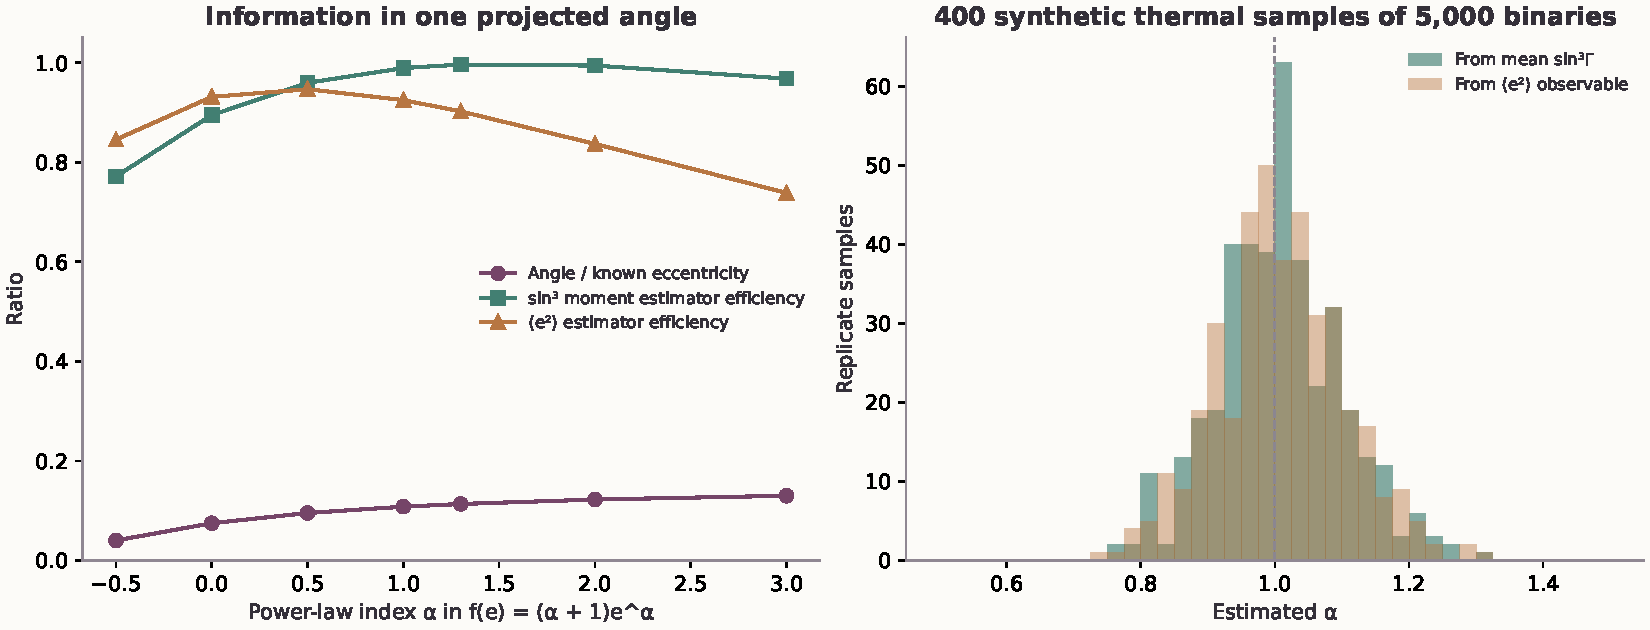
\includegraphics[width=\linewidth]{figures/powerlaw_index_information.pdf}
\caption{Left: information in one ideal projected angle about $\alpha$, relative to a directly measured eccentricity, and the asymptotic efficiencies of the two moment estimators \eqref{eq:alphahat}. Right: estimates of $\alpha$ from $400$ synthetic thermal samples ($\alpha=1$, dashed) of $5\,000$ independent Kepler-simulated binaries each.}\label{fig:fisher}
\end{figure}

\section{Which selections keep the model exact}\label{sec:selection}

Real samples are selected, for example by projected separation, by the significance of the measured relative motion and by contamination cuts. In general, let $z$ collect the latent orbital variables, let $y$ be the measured data with law $R(\dd y\mid z)$, let $S(y,z)$ be the probability of selection, and let $\gamma(y)$ be the measured angle. The observed law is
\begin{equation}\label{eq:obsmodel}
P_{\rm obs}(A)=\frac{\iint\ind_{\{\gamma(y)\in A\}}\,S(y,z)\,R(\dd y\mid z)\,P_F(\dd z)}{\iint S(y,z)\,R(\dd y\mid z)\,P_F(\dd z)}.
\end{equation}
Selection can change both the eccentricity mixture and the angle law at fixed eccentricity. Selection on the same noisy measurement that yields the angle is included. The angle-only selection of Section~\ref{sec:stability} is the special case without measurement error in which $S$ depends only on $\Gamma$. Two other cases are exact and directly relevant to Gaia samples.

\begin{proposition}[Thermal populations are immune to azimuth-blind selection]\label{prop:thermal}
Suppose that, conditional on semimajor axis and total mass, the population is thermal with uniform mean anomaly and Haar orientation. Let the selection probability be a measurable function of the semimajor axis, the total mass, the true lengths $|\bm r|$ and $|\bm v|$, and the angles that $\bm r$ and $\bm v$ make with the line of sight (hence of projected separation, projected speed and radial velocity), with positive expectation. It must not depend on either sky position angle. Then the selected projected angle is exactly uniform on $[0,\pi]$. Further covariates, such as the mass ratio, may enter the selection only if the orbital law is also thermal conditional on them.
\end{proposition}

\begin{proof}
At fixed semimajor axis and mass, a thermal population with uniform mean anomaly and Haar orientation is the microcanonical distribution, the normalised Liouville measure $\delta\big(|\bm v|^2/2-\mu/|\bm r|-E_0\big)\dd^3r\,\dd^3v$ \citep{Jeans1919,Hwang2022}. (In Delaunay variables, fixing the energy fixes $L$, and integrating the normal component of angular momentum over $[-G,G]$ leaves the weight $2G\dd G$ with $G=L\sqrt{1-e^2}$, which is the thermal law.) Its density depends on $(\bm r,\bm v)$ only through $|\bm r|$ and $|\bm v|$, so conditional on these lengths the directions $\widehat{\bm r}$ and $\widehat{\bm v}$ are independent and uniform on the sphere. For a uniform direction, the polar angle from the line of sight and the sky position angle are independent, and the position angle is uniform. The four angles are therefore independent, the two position angles are uniform, and the selection depends only on the other variables. The projected angle is the difference of the two position angles, folded into $[0,\pi]$, which is uniform. Mixing over semimajor axes and masses preserves uniformity.
\end{proof}

\citet{Hwang2022} found numerically that the thermal angle law stays flat under every velocity criterion they tried; Proposition~\ref{prop:thermal} proves this. With Theorem~\ref{thm:inverse} it gives a selection-robust test. A significantly non-uniform angle law in a subsample selected as in Proposition~\ref{prop:thermal} rejects the conditional thermal null (thermal at each semimajor axis and total mass, with phase mixing and isotropy). It does not reject marginal thermality on its own, since a population can be thermal overall but not at each semimajor axis. Selections that do use position angles, such as Gaia's scan-law dependent resolution of close pairs \citep{Hwang2022}, are not covered, nor are cuts on measured quantities whose errors depend on position angle.

\begin{proposition}[Binning by projected separation]\label{prop:sbin}
Let $z$ collect eccentricity, phase and orientation, with probability law $P_z$, and let the parent population be the $\sigma$-finite product measure $a^{-\beta}\dd a\,P_z(\dd z)$ on $(0,\infty)\times\{z\}$. Write $\rho=s/a$, where $s$ is the projected separation; $\rho=\rho(z)$ depends only on $z$. For a bin $B$ with $0<\int_Bs^{-\beta}\dd s<\infty$ and $0<\E\rho^{\beta-1}<\infty$, the normalised law of $z$ among systems with $s\in B$ is $P_z$ reweighted by $\rho^{\beta-1}$. In particular, for \"Opik's law $\beta=1$, every projected-separation bin has the original eccentricity law, phase law and orientation law, and Theorems~\ref{thm:kernel}--\ref{thm:moments} apply within each bin without change.
\end{proposition}

\begin{proof}
For fixed $z$, the substitution $s=a\rho(z)$ maps $a^{-\beta}\dd a$ to $\rho(z)^{\beta-1}s^{-\beta}\dd s$. Hence the parent measure becomes $s^{-\beta}\dd s\,\rho(z)^{\beta-1}P_z(\dd z)$, a product of a function of $s$ and a measure in $z$. Restricting to $s\in B$ gives total mass $\int_Bs^{-\beta}\dd s\cdot\E\rho^{\beta-1}$, finite and positive by assumption, and normalising leaves $\rho^{\beta-1}P_z/\E\rho^{\beta-1}$ as the law of $z$.
\end{proof}

The proposition is exact only for a scale-free semimajor-axis law over an unbounded range. Table~\ref{tab:sbin} shows what happens with a finite range, $a\in[10,10^6]$, a realistic bin $10^3<s<10^{3.5}$ and the slopes $\beta=1.6$ and $2$ that describe the observed steepening of the separation distribution at large separations \citep{ElBadry2021}. With a finite range the exact weight also depends on $z$ through the overlap of $B$ with $[a_{\min}\rho,a_{\max}\rho]$, so the scale-free prediction in the table is an approximation; it is accurate when the bin lies far inside the range. The sample mean of $W_1$ follows it. At $\beta=1$ it recovers the parent mean circularity, and at $\beta=1.6$ the resulting bias in $\alpha$ is at most a few hundredths. The bias is not the change in the binned eccentricity law alone, because selection also changes the angle law at fixed eccentricity. A cut on projected speed is not covered by Proposition~\ref{prop:sbin} unless the population is thermal, and it can distort non-thermal angle laws strongly. Orientation is also an assumption: Galactic tides can make the orientations of the widest binaries anisotropic \citep{Hamilton2022}.

\begin{table}[tb]
\centering
\caption{Binning by projected separation, $10^3<s<10^{3.5}$, with $dN/da\propto a^{-\beta}$ on $[10,10^6]$ (units arbitrary) and $2\times10^6$ Kepler-simulated binaries per row. ``Parent'' is the analytic mean circularity of the power law; ``in bin'' is the mean over the simulated eccentricities in the bin. ``Prediction'' is the $\rho^{\beta-1}$-reweighted expectation of $W_1$ from Proposition~\ref{prop:sbin}. Standard errors of $\overline{W_1}$ are given in brackets.}\label{tab:sbin}
\begin{tabular}{rrrrrrrr}
\toprule
$\alpha$ & $\beta$ & $N$ in bin & Parent $\E j$ & In-bin $\E j$ & $\overline{W_1}$ (s.e.) & Prediction & $\widehat\alpha_{\sin^3}$\\
\midrule
0 & 1 & 199,889 & 0.7854 & 0.7852 & 0.7846 (0.0013) & 0.7847 & 0.005\\
0 & 1.6 & 58,141 & 0.7854 & 0.7686 & 0.7903 (0.0024) & 0.7917 & -0.032\\
0 & 2 & 12,612 & 0.7854 & 0.7571 & 0.7931 (0.0052) & 0.7925 & -0.050\\
1.3 & 1 & 199,522 & 0.6403 & 0.6406 & 0.6402 (0.0013) & 0.6403 & 1.301\\
1.3 & 1.6 & 61,172 & 0.6403 & 0.6263 & 0.6407 (0.0023) & 0.6394 & 1.294\\
1.3 & 2 & 13,764 & 0.6403 & 0.6144 & 0.6486 (0.0048) & 0.6413 & 1.201\\
\bottomrule
\end{tabular}
\end{table}

\section{Identifiability has a stability limit}\label{sec:stability}

\begin{proposition}[Discontinuity in total variation]\label{prop:TV}
Fix $0<\varepsilon<1$ and consider the eccentricity densities
\begin{equation}
f_n^{\pm}(e)=2e\,[1\pm\varepsilon\cos(2\pi n e^2)],\qquad n\ge1.
\end{equation}
Their total-variation distance is $2\varepsilon/\pi$ for every $n$, whereas the total-variation distance between their projected-angle laws tends to zero. Here $\TV(P,Q)=\tfrac12\int|p-q|$.
\end{proposition}

\begin{proof}
Both densities are nonnegative and normalised. With $u=e^2$,
\begin{equation}
\TV(F_n^+,F_n^-)=\varepsilon\int_0^1|\cos(2\pi n u)|\dd u
=\frac{2\varepsilon}{\pi}.
\end{equation}
Their angle densities are $p_n^{\pm}=\pi^{-1}\pm\varepsilon h_n$, where
\begin{equation}
h_n(\gamma)=\int_0^1K(\gamma,\sqrt u)\cos(2\pi n u)\dd u.
\end{equation}
For almost every $\gamma$, the kernel in this integral is integrable in $u$, with integral $1/\pi$ by the thermal identity. The Riemann--Lebesgue lemma gives $h_n(\gamma)\to0$ and positivity gives $|h_n(\gamma)|\le1/\pi$. Dominated convergence therefore implies $\varepsilon\int_0^\pi|h_n|\dd\gamma\to0$, which is the angle total-variation distance.
\end{proof}

Indeed, each $F_n^+$ remains at distance $\varepsilon/\pi$ from the thermal law, while its angle law converges in total variation to uniform. Thus the inverse is discontinuous even at that benchmark. No uniformly accurate total-variation reconstruction of arbitrary fine density structure follows from the uniqueness theorem. The bounded moment estimators remain valid because they target specified functionals. The mechanism---oscillatory perturbations annihilated in the limit by an integrable kernel---is the standard one for smoothing operators and Abel equations \citep{GorenfloVessella1991}; the proposition records its explicit form for this orbital observable rather than a new instability principle.

Numerically, the angle distance in this family decays like $1/n$ (Section~\ref{sec:numerics}): $n$ times the distance stays between $0.091$ and $0.101$ for $n=1,2,4,\ldots,64$. Most of it comes from nearly aligned angles, where the Jacobian $1/(1-c^2)$ makes the forward map least smoothing. We do not prove a rate, a modulus of continuity or a minimax bound.

The failure is specific to strong metrics. Informally, total variation is sensitive to every fine difference between two distributions, whereas weak convergence asks only that broad features, such as averages of smooth functions or cumulative probabilities, agree. On the closure $[0,1]$, with the radial law $\tfrac12\delta_0+\tfrac12\delta_\pi$ at $e=1$, the inverse is continuous for weak convergence.

\begin{proposition}[Weak continuity of the inverse]\label{prop:weak}
Let $\mathcal P[0,1]$ carry the weak topology. The map $F\mapsto P_F$ from eccentricity laws to angle laws is continuous and injective, so its inverse is continuous on its image. In particular, if $P_{F_n}\to P_F$ weakly, then $F_n\to F$ weakly, and $F_n([0,r))\to F([0,r))$ at every $r$ with $F(\{r\})=0$.
\end{proposition}

\begin{proof}
Use the representation in the proof of Theorem~\ref{thm:kernel}: with $\beta$ uniform and $U$ uniform on $[-1,1]$ independently, $T=j|\sin\beta|$ and $\Gamma=\operatorname{atan2}\big(T,U\sqrt{1-T^2}\big)$ has law $P_e$, and at $e=1$ this gives the radial law. For fixed $(\beta,U)$ with $U\ne0$ and $\sin\beta\ne0$, $\Gamma$ is a continuous function of $e\in[0,1]$. For bounded continuous $\varphi$, dominated convergence makes $e\mapsto\int\varphi\dd P_e$ bounded and continuous, so $F\mapsto\int\varphi\dd P_F=\int\!\int\varphi\dd P_e\,F(\dd e)$ is weakly continuous. Injectivity on $[0,1]$ is Theorem~\ref{thm:inverse} together with the recovery of the radial atom from the mass at $\{0,\pi\}$ (Section~\ref{sec:inverse}). A continuous injection from the compact space $\mathcal P[0,1]$ into a Hausdorff space is a homeomorphism onto its image.
\end{proof}

Weak continuity gives no rate, and finite samples still cannot resolve atoms or sharp features reliably. It does explain why broad features such as cumulative probabilities at continuity points are recoverable. A nonparametric maximum-likelihood fit on a grid recovers them in simulations (Section~\ref{sec:numerics}).

\subsection{Known error and known selection}

There are limited extensions that preserve identifiability. Regard the symmetric angle law as a law modulo $\pi$. Independent known circular angular error multiplies Fourier coefficient $k$ by its known multiplier $\widehat h_k$. If every multiplier is nonzero, equality of noisy laws forces equality of the error-free laws and then of $F$. Wrapped Gaussian error with variance $\sigma^2$ has multiplier $\exp(-2k^2\sigma^2)$, so it preserves uniqueness but makes fine-scale inversion much less stable. This additive circular model is not a substitute for a full Gaia proper-motion error model.

If selection depends only on the true angle through a known positive function $s(\gamma)$, then $p_{\rm sel}\propto s p_F$ can be inverted by normalised division by $s$. Selection with zero-probability regions, unknown selection, or selection on latent phase and orientation is not covered by this statement. A concrete warning is selection on true separation $r>a$: since $r/a=1-e\cos E$, it keeps exactly the phases with $\cos E<0$, the selected law of $\sin E$ is no longer that of uniform $E$, and the phase-pairing step \eqref{eq:phasepair} fails. Projected-separation cuts act similarly. Exactly edge-on orientations make the angle distribution concentrate at $0$ and $\pi$ for every eccentricity, illustrating failure of uniqueness without the orientation assumption.

\section{Reproducible numerical checks}\label{sec:numerics}

All catalogues in this section are synthetic, and every pass/fail check is an explicit test that also runs under \texttt{python -O}. The supplied module evaluates the exact likelihood stably, evaluates the power-law family, computes the bounded observables and confidence intervals, and samples either the proven mixture or independent Kepler orbits. The validation uses the latter: it solves $E-e\sin E=M$, rotates both orbital vectors with independent uniform pericentre and uniform $\cos i$, and measures the angle with dot and cross products. It never calls the analytic likelihood to generate its physical simulations.

\subsection{Deterministic integration and independent simulations}

Deterministic quadrature checked normalisation at eight eccentricities from zero to $0.9999$, and moments $k=1,2,3,6,12$. Maximum observed discrepancies were of order $10^{-14}$ for normalisation and $10^{-13}$ for the moment identities. The fractional identities \eqref{eq:moment} at $s\in\{0.25,0.5,1,2,3.5,6\}$ and the Fourier identities \eqref{eq:e2}--\eqref{eq:e4} agree to $3\times10^{-14}$ at five eccentricities, and the stated observable ranges were confirmed on a dense grid. These are floating-point agreement figures, not certified error bounds. Additional checks compare \eqref{eq:powerlaw} with numerical eccentricity mixtures and differentiate the fixed-eccentricity kernel away from its cusp.

The inverse \eqref{eq:inverse} was run end to end. Starting only from a mixed angle density, the check differentiates $Y_F$ numerically and evaluates the inverse integral. It recovers $F([0,r))$ for an atomic law (atoms $0,0.35,0.8$ with weights $0.2,0.5,0.3$; the atom locations are supplied to the quadrature as breakpoints) and for three power laws to within $3.1\times10^{-4}$ at points away from the atoms.

The physical simulation uses $400\,000$ binaries at each of five eccentricities, for $2\,000\,000$ independent cases. Across the first six moment observables in each case, the largest standardised discrepancy is below $1.854$ estimated standard errors. The 24-bin angle checks are reported in full in Table~\ref{tab:mc}. Their pooled statistic is $119.985$ on 115 degrees of freedom ($p=0.356$). Binning-free Kolmogorov--Smirnov tests against the exact distribution function give $p$ values $0.734$, $0.790$, $0.025$, $0.219$, $0.646$ at the five eccentricities of Table~\ref{tab:mc}; the run is gated at a family-wise level of $0.001$ over all ten tests. Two phase controls test the reduction directly. Uniform eccentric anomaly, which satisfies the pairing condition of Section~\ref{sec:model}, agrees with the kernel ($p=0.81$ and $0.20$ at $e=0.6$ and $0.9$). Uniform true anomaly, which does not, is rejected ($\chi^2=959$ and $43\,033$ on 23 degrees of freedom). The new observables were also checked against the Kepler simulator at $e\in\{0,0.6,0.95\}$ with $400\,000$ binaries each; the largest standardised discrepancy was $2.89$ over twelve comparisons. These consistency checks supplement the analytic proofs.

\begin{table}[tb]
\centering
\caption{Independent Kepler simulations: 24 angular bins, with exact integrated bin probabilities. The five $p$ values are unadjusted. The smallest is below $0.05$, which is unremarkable among ten tests, and well above the pre-registered gate.}\label{tab:mc}
\begin{tabular}{rrrr}
\toprule
$e$ & Number of binaries & $\chi^2$ (23 d.f.) & $p$\\
\midrule
0 & 400,000 & 19.081 & 0.696\\
0.3 & 400,000 & 15.385 & 0.880\\
0.6 & 400,000 & 23.119 & 0.454\\
0.9 & 400,000 & 25.589 & 0.321\\
0.99 & 400,000 & 36.810 & 0.034\\
\bottomrule
\end{tabular}
\end{table}

\begin{figure}[tb]
\centering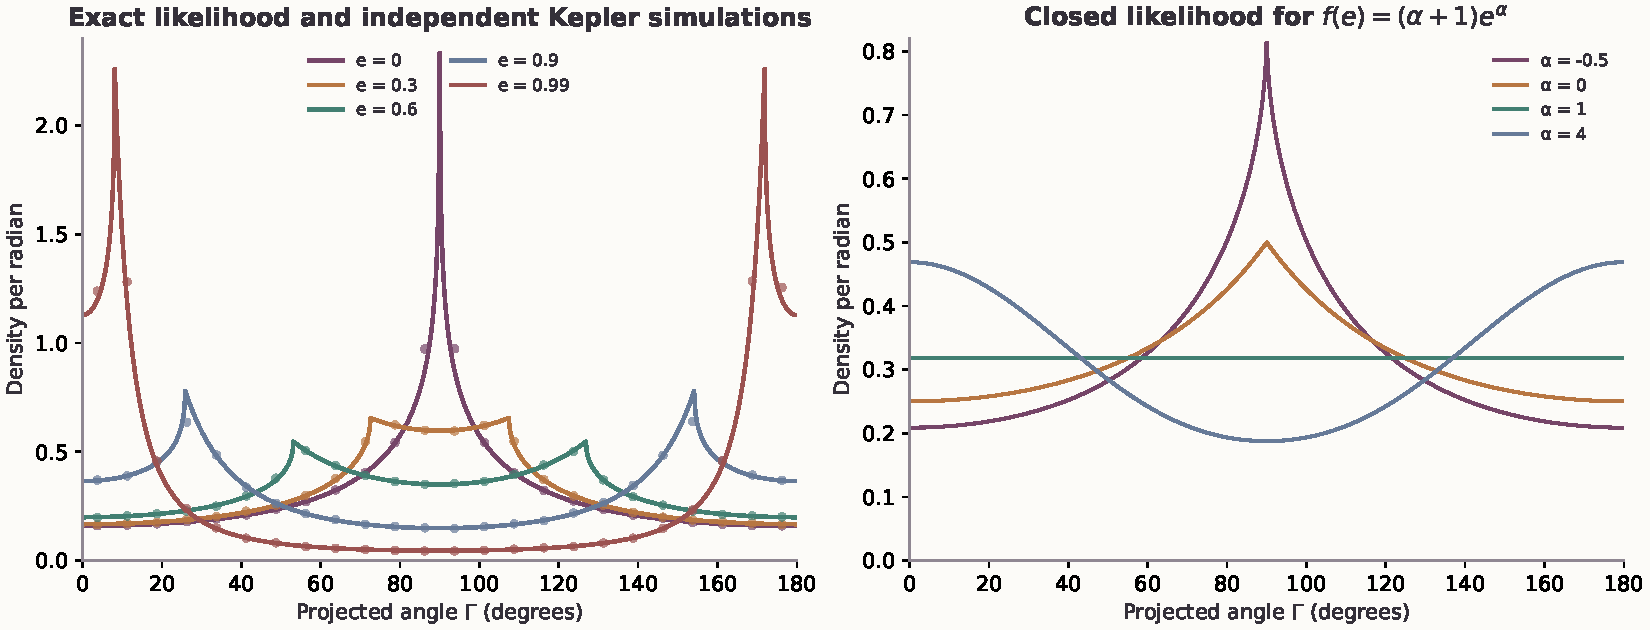
\includegraphics[width=\linewidth]{figures/likelihood_validation.pdf}
\caption{Left: exact densities and independent Kepler-simulation bin averages, shown as points. The circular logarithmic peak is truncated by the plotting range; bin averages need not lie on a sharply curved pointwise density. Right: the closed power-law family. All plotted densities are per radian although the horizontal coordinate is labelled in degrees.}\label{fig:likelihood}
\end{figure}

\subsection{Moment recovery and assumption sensitivity}

A separate $20\,000$-binary experiment uses a discrete population with eccentricities $(0,0.65,0.95)$ and weights $(0.2,0.5,0.3)$. The module estimates the first six odd circularity moments and records their sample covariance, standard errors and simultaneous Hoeffding intervals. Figure~\ref{fig:sensitivity} compares estimates with their exact population targets. Its displayed $1.96$-standard-error bars are descriptive normal-approximation intervals; the JSON results also contain the distribution-free simultaneous intervals.

Sensitivity experiments hold $e=0.6$, hence true $j=0.8$, fixed. They are deliberately extreme and use latent quantities: the separation cut below uses the true semimajor axis, which an observer does not know, and Table~\ref{tab:sbin} gives the realistic version. An inclination restriction $|\cos i|<0.2$ changes the mean-moment estimate to $0.212$; $|\cos i|>0.8$ gives $1.127$, beyond the admissible population range. Selecting projected separation above $1.1a$ gives $0.886$. Uniform true anomaly gives $0.820$. Additive angular errors with standard deviations $10^\circ$ and $30^\circ$ give $0.792$ and $0.745$. These deliberately strong interventions illustrate scope and bias; they are not estimates of selection or error in an actual catalogue.

\begin{figure}[tb]
\centering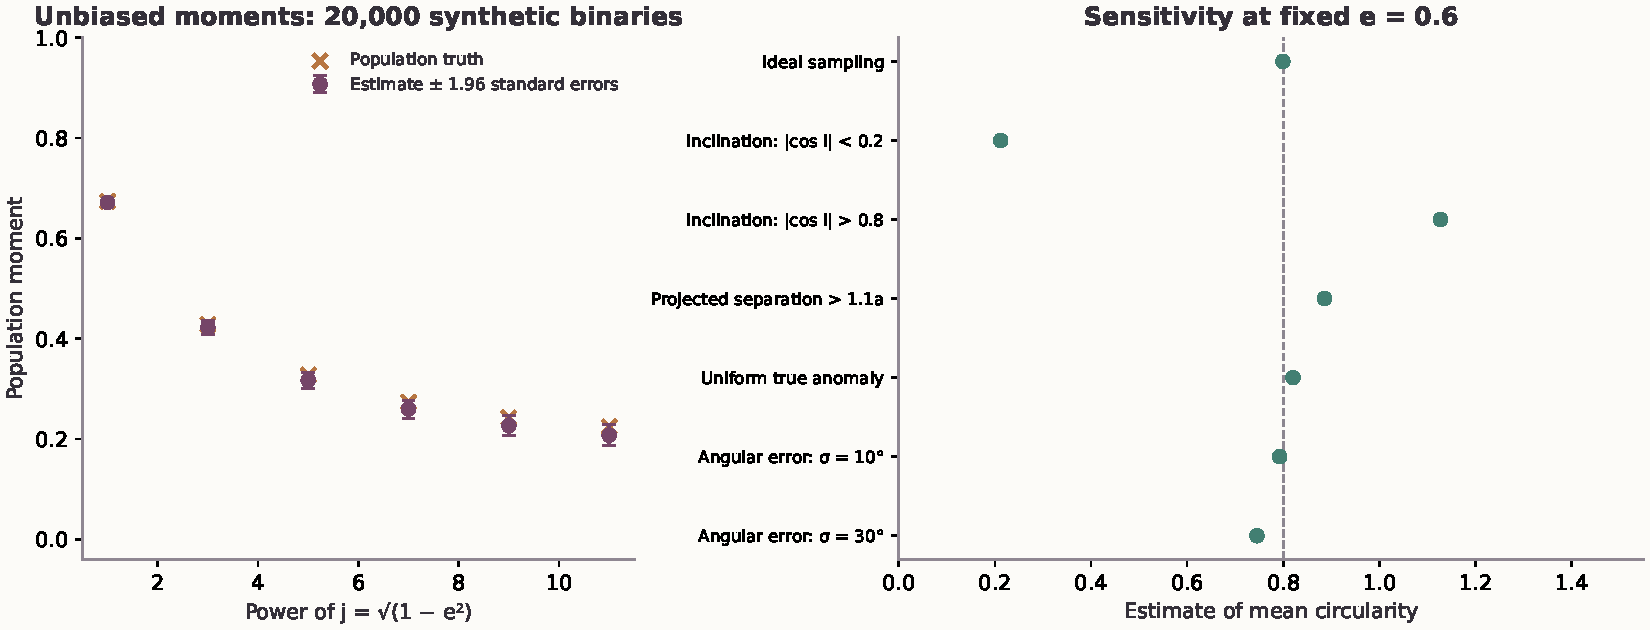
\includegraphics[width=\linewidth]{figures/moments_and_sensitivity.pdf}
\caption{Left: six odd circularity moments in the synthetic discrete-mixture benchmark. Right: raw estimates at fixed $e=0.6$ after changing the sampling or adding angular error. The dashed line marks the true circularity $0.8$. Point estimates are not clipped to the model range; a value above one is informative about assumption failure.}\label{fig:sensitivity}
\end{figure}

\subsection{Selection and a finite-sample estimator}

Proposition~\ref{prop:thermal} was checked on $2\times10^6$ thermal binaries with log-uniform semimajor axes. Within the bin $10^3<s<10^{3.5}$ the angle law is flat ($p=0.34$, $N=199\,996$), and it stays flat after also keeping only the half with larger $v_{\rm proj}\sqrt s$, the projected speed in units of the circular speed at the projected separation ($p=0.10$, $N=99\,998$). Table~\ref{tab:sbin} reports the separation-binning experiment.

To show that identifiability can be turned into a working estimator, an approximate grid maximum-likelihood fit (EM on 201 eccentricities in $[0,0.995]$, using the exact kernel, with its convergence and optimality residual recorded) was applied to Kepler-simulated samples from a population with three parts: 30\% uniform on $[0.1,0.4]$, 50\% thermal and a 20\% atom at $e=0.9$. The largest error in the fitted step distribution function at six fixed points was $0.103$, $0.061$, $0.036$ for $N=2\,000$, $20\,000$ and $100\,000$, respectively. EM stopped at its 5\,000-iteration cap with optimality residual below $2\times10^{-4}$ in all three runs (the residual is zero at the exact grid maximum), and no kernel values were capped. The fitted mean circularity agreed with the direct estimate $\overline{W_1}$ to within $0.001$. The estimator is a demonstration; its consistency and rate are not proved here.

\subsection{Visible inverse instability}

For Proposition~\ref{prop:TV}, take $\varepsilon=0.75$. The latent total-variation distance stays at $0.477465$. The corresponding angle distances are approximately $0.0987$ at $n=1$, $0.05034$ at $n=2$, $0.01223$ at $n=8$, $0.002922$ at $n=32$ and $0.001433$ at $n=64$; $n$ times the distance stays between $0.091$ and $0.101$ at the seven tested frequencies $n=1,2,4,\ldots,64$. Figure~\ref{fig:instability} displays the contrast. The numerical calculation uses a Fresnel representation of the Abel integral and dense deterministic integration, separately from the theorem's convergence argument.

\begin{figure}[tb]
\centering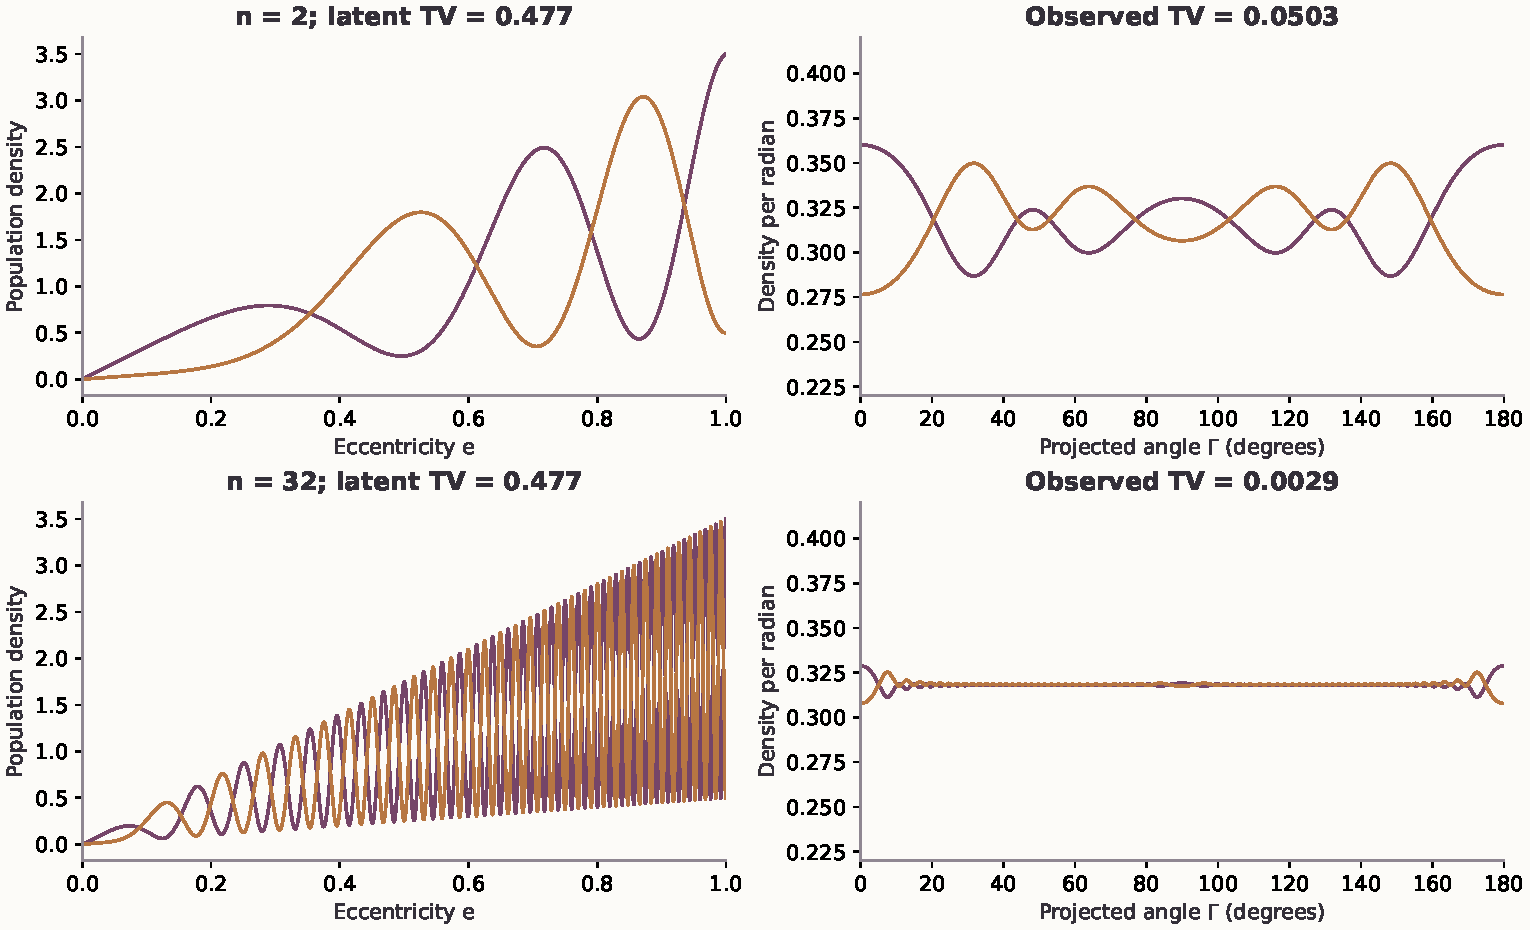
\includegraphics[width=.96\linewidth]{figures/inverse_instability.pdf}
\caption{Different eccentricity laws can produce very similar angle densities. The left-hand distributions remain equally separated in total variation as oscillation frequency rises, while their projected laws approach each other. This illustrates a proved instability, not a counterexample to exact identifiability.}\label{fig:instability}
\end{figure}

\section{What the result establishes}

For the ideal Keplerian population, Theorem~\ref{thm:kernel} gives the projected-angle likelihood in closed form, and Theorem~\ref{thm:inverse} shows that the angle law determines the eccentricity law exactly. That answers the uniqueness question of \citet{Hwang2022} Appendix~B. Their suspicion of approximate uniqueness is right in the weak topology (Proposition~\ref{prop:weak}) and wrong in total variation (Proposition~\ref{prop:TV}).

For practice, the most useful results are the estimators that need no fitting. Mean circularity and mean square eccentricity are sample means of explicit bounded functions of the angle, and power-law indices in both common parametrisations are explicit functions of such means (Theorem~\ref{thm:moments}, Corollary~\ref{cor:even}, equations \eqref{eq:alphahat} and \eqref{eq:makarov}). Theorem~\ref{thm:dual} shows that the moment observables are the only symmetric unbiased single-angle observables for their targets. Under the ideal model the simplest of them is nearly efficient for $\alpha$, and near the thermal law one angle is worth about a ninth of a measured eccentricity for this parameter.

Two selection results say when the ideal model survives observation. Populations that are thermal at each semimajor axis and total mass keep an exactly uniform angle law under selection on true lengths, line-of-sight angles, semimajor axis and total mass, but not on sky position angles (Proposition~\ref{prop:thermal}). Binning by projected separation is exact when semimajor axes follow a scale-free \"Opik law independent of the orbital shape, phase and orientation, and is otherwise an explicit reweighting; with a finite range of semimajor axes it holds only approximately, and well only when the bin lies far from the ends of the range (Proposition~\ref{prop:sbin}, Table~\ref{tab:sbin}). Everything else, including significance cuts on the measured motion for non-thermal populations, heteroscedastic astrometric errors, contamination and anisotropic orientations, needs the observation model \eqref{eq:obsmodel}.

Several tasks remain open. An analysis of a real catalogue such as that of \citet{ElBadry2021} would need a vector proper-motion error model inside \eqref{eq:obsmodel}. The grid maximum-likelihood fit needs a consistency and rate theory, which the Wicksell literature suggests is attainable \citep{GroeneboomJongbloed1995}. The $1/n$ attenuation needs a proof. A closed joint law for the angle together with a speed variable, in the spirit of the angle-and-speed method of \citet{TokovininKiyaeva2016} and the speed distributions of \citet{Benisty2022}, would show how much extra stability speed buys. The accompanying bounded novelty audit found no equivalent result in the inspected literature through 31 October 2026. It records its sources and the older stereology texts it could not inspect.

\appendix
\section{A flat-prior posterior in closed form}

This appendix illustrates the likelihood; a flat eccentricity prior is a choice, not a claim about any stellar population. For $c=|\cos\gamma|<1$ and prior density one, normalisation uses $p_0(\gamma)$ from \eqref{eq:instances}. For every real $m\ge0$,
\begin{equation}
\E[e^m\mid\gamma]=
\frac{B((m+1)/2,1/2)}{\pi(m+1)}
\frac{1-c^{m+1}}{1-c}.
\end{equation}
This follows by dividing $p_m(\gamma)/(m+1)$ by $p_0(\gamma)$. In particular,
\begin{equation}
\E[e\mid\gamma]=\frac{1+c}{\pi}.
\end{equation}
For $a>0$, define
\begin{equation}
L_a(r)=
\begin{cases}
r\acosh(a/r)+a\arcsin(r/a),&0<r<a,\\
a\pi/2,&r\ge a,
\end{cases}
\end{equation}
with $L_a(0)=0$ and $L_0=0$. Since $L_a(r)=\int_0^{\min(r,a)}\acosh(a/e)\dd e$, the posterior cumulative distribution is
\begin{equation}
\Prob(e\le r\mid\gamma)=\frac{2[L_1(r)-L_c(r)]}{\pi(1-c)},\qquad 0\le r\le1.
\end{equation}
The limiting posterior at angular endpoints is $(2/\pi)\arcsin r$. The uniform-prior mode $e=c$ is the earlier modal observation credited in Section 3. To verify the mode as a function of eccentricity, for $0<e<c<1$ the derivative of the kernel numerator is
\begin{equation}
\frac1e\left[\frac{c}{\sqrt{c^2-e^2}}-\frac1{\sqrt{1-e^2}}\right]>0,
\end{equation}
whereas for $c<e<1$ the derivative is $-1/(e\sqrt{1-e^2})<0$. At $c=0$ the maximum is the circular endpoint. A population-identifiability theorem does not make this individual posterior concentrated.

\section{Stable evaluation and reproducibility}

For $c>e$, evaluate the inverse-hyperbolic difference as
\begin{equation}
\log\frac{1+\sqrt{1-e^2}}{c+\sqrt{c^2-e^2}}.
\end{equation}
Near angular endpoints the implementation further rationalises its numerator and uses \texttt{log1p} to avoid subtracting nearly equal quantities. The power-law implementation uses \texttt{expm1} for $1-c^{\alpha+1}$ and evaluates $\log c$ directly near $\pi/2$, where computing it from $\sin^2\gamma$ would lose precision.

The reproducibility package contains \texttt{wide\_binary\_angles.py} (likelihoods, observables, estimators and simulators), \texttt{validate\_and\_plot.py} (all checks, tables and figures), a negative-control script, the proof notes, numerical outputs, figures and the novelty report. Run
\begin{quote}
\verb|python validate_and_plot.py --n-per-e 400000 --out replay|
\end{quote}
with NumPy~2.3.5, SciPy~1.17.0 and Matplotlib~3.10.8. The seed is 20261028, the run takes a few minutes, and \texttt{--out} keeps the shipped results unchanged. Every check raises an error on failure, also under \texttt{python -O}; the negative-control script confirms that deliberately corrupted kernels, observables and simulators are caught. The package contains no observational stellar catalogue and no copies of cited papers. The archived package is deposited at \url{https://doi.org/10.5281/zenodo.23838665} (all versions: \url{https://doi.org/10.5281/zenodo.23838664}), with source at \url{https://github.com/ipitchford/wide-binary-angle-inversion}.

\begin{thebibliography}{99}
\bibitem[Brandt(2026)]{Brandt2026}
Brandt, T. D. (2026). \emph{Closed-form statistical relations between projected separation, semimajor axis, companion mass, and host acceleration}. arXiv:2601.14688v2. \url{https://arxiv.org/abs/2601.14688}

\bibitem[Benisty et al.(2022)]{Benisty2022}
Benisty, D., Evans, N. W., \& Davis, A.-C. (2022). The eccentricity distribution of wide binaries. \emph{Monthly Notices of the Royal Astronomical Society: Letters, 518}(1), L51--L56. \url{https://doi.org/10.1093/mnrasl/slac134}

\bibitem[Bhatia and Davis(2000)]{BhatiaDavis2000}
Bhatia, R., \& Davis, C. (2000). A better bound on the variance. \emph{The American Mathematical Monthly, 107}(4), 353--357. \url{https://doi.org/10.1080/00029890.2000.12005203}

\bibitem[El-Badry et al.(2021)]{ElBadry2021}
El-Badry, K., Rix, H.-W., \& Heintz, T. M. (2021). A million binaries from Gaia eDR3: sample selection and validation of Gaia parallax uncertainties. \emph{Monthly Notices of the Royal Astronomical Society, 506}(2), 2269--2295. \url{https://doi.org/10.1093/mnras/stab323}

\bibitem[Gorenflo and Vessella(1991)]{GorenfloVessella1991}
Gorenflo, R., \& Vessella, S. (1991). \emph{Abel Integral Equations: Analysis and Applications}. Lecture Notes in Mathematics, Springer. \url{https://doi.org/10.1007/BFb0084665}

\bibitem[Groeneboom and Jongbloed(1995)]{GroeneboomJongbloed1995}
Groeneboom, P., \& Jongbloed, G. (1995). Isotonic estimation and rates of convergence in Wicksell's problem. \emph{The Annals of Statistics, 23}(5), 1518--1542. \url{https://doi.org/10.1214/aos/1176324310}

\bibitem[Hamilton(2022)]{Hamilton2022}
Hamilton, C. (2022). On the phase-mixed eccentricity and inclination distributions of wide binaries in the Galaxy. \emph{The Astrophysical Journal Letters, 929}(2), L29. \url{https://doi.org/10.3847/2041-8213/ac6600}

\bibitem[Hausdorff(1923)]{Hausdorff1923}
Hausdorff, F. (1923). Momentprobleme f\"ur ein endliches Intervall. \emph{Mathematische Zeitschrift, 16}(1), 220--248. \url{https://doi.org/10.1007/BF01175684}

\bibitem[Hwang et al.(2022a)]{Hwang2022}
Hwang, H.-C., Ting, Y.-S., \& Zakamska, N. L. (2022a). The eccentricity distribution of wide binaries and their individual measurements. \emph{Monthly Notices of the Royal Astronomical Society, 512}(3), 3383--3399. \url{https://doi.org/10.1093/mnras/stac675}

\bibitem[Hwang et al.(2022b)]{Hwang2022twin}
Hwang, H.-C., El-Badry, K., Rix, H.-W., Hamilton, C., Ting, Y.-S., \& Zakamska, N. L. (2022b). Wide twin binaries are extremely eccentric: evidence of twin binary formation in circumbinary disks. \emph{The Astrophysical Journal Letters, 933}(2), L32. \url{https://doi.org/10.3847/2041-8213/ac7c70}

\bibitem[Hwang(n.d.)]{HwangCode}
Hwang, H.-C. (n.d.; accessed 28 October 2026). \emph{Eccentricity-of-wide-binaries: Public code and simulation grids}, README. \url{https://github.com/HC-Hwang/Eccentricity-of-wide-binaries}

\bibitem[Hoeffding(1963)]{Hoeffding1963}
Hoeffding, W. (1963). Probability inequalities for sums of bounded random variables. \emph{Journal of the American Statistical Association, 58}(301), 13--30. \url{https://doi.org/10.1080/01621459.1963.10500830}

\bibitem[Jeans(1919)]{Jeans1919}
Jeans, J. H. (1919). The origin of binary systems. \emph{Monthly Notices of the Royal Astronomical Society, 79}(6), 408--416. \url{https://doi.org/10.1093/mnras/79.6.408}

\bibitem[Kloza and Elliott(2023)]{Kloza2023}
Kloza, P. A., \& Elliott, J. A. (2023). Inverse projection of axisymmetric orientation distributions. \emph{EPL, 143}, 22002. \url{https://doi.org/10.1209/0295-5075/ace4ee}

\bibitem[Makarov(2025a)]{Makarov2025}
Makarov, V. V. (2025a). Distributions of wide binary stars in theory and in Gaia data. I. Generalized Ambartsumian (1937) approach and the family of power-law distributions of eccentricity. \emph{The Astronomical Journal, 169}(2), 113. \url{https://doi.org/10.3847/1538-3881/ada5fa}

\bibitem[Makarov(2025b)]{Makarov2025b}
Makarov, V. V. (2025b). Distributions of wide binary stars in theory and in Gaia data. II. Reconstruction of sample probability density of true orbit sizes. \emph{The Astronomical Journal, 170}(3), 138. \url{https://doi.org/10.3847/1538-3881/adec79}

\bibitem[Makarov(2026)]{Makarov2025c}
Makarov, V. V. (2026). Distributions of wide binary stars in theory and in Gaia data. III. Orbital momenta, masses, and manifestations of MOND. \emph{The Astronomical Journal, 171}(2), 79. \url{https://doi.org/10.3847/1538-3881/ae2757}

\bibitem[Shatsky(2001)]{Shatsky2001}
Shatsky, N. (2001). The long-period companions of multiple stars tend to have moderate eccentricities. \emph{Astronomy \& Astrophysics, 380}(1), 238--244. \url{https://doi.org/10.1051/0004-6361:20011401}

\bibitem[Tokovinin(1998)]{Tokovinin1998}
Tokovinin, A. A. (1998). On the distribution of orbital eccentricities for wide visual binary stars. \emph{Astronomy Letters, 24}(2), 178--179. Complete public scan consulted: \url{https://articles.adsabs.harvard.edu/pdf/1998AstL...24..178T}

\bibitem[Tokovinin and Kiyaeva(2016)]{TokovininKiyaeva2016}
Tokovinin, A., \& Kiyaeva, O. (2016). Eccentricity distribution of wide binaries. \emph{Monthly Notices of the Royal Astronomical Society, 456}(2), 2070--2079. \url{https://doi.org/10.1093/mnras/stv2825}

\bibitem[Tokovinin(2020)]{Tokovinin2020}
Tokovinin, A. (2020). Eccentricity distribution of wide low-mass binaries. \emph{Monthly Notices of the Royal Astronomical Society, 496}(1), 987--993. \url{https://doi.org/10.1093/mnras/staa1639}
\bibitem[Wicksell(1925)]{Wicksell1925}
Wicksell, S. D. (1925). The corpuscle problem. A mathematical study of a biometric problem. \emph{Biometrika, 17}(1--2), 84--99. \url{https://doi.org/10.1093/biomet/17.1-2.84}
\end{thebibliography}
\end{document}
